% -------------------------------------------------------------------------
% LaTeX Vorlage für wissenschaftliche Arbeiten am IGMR 
% LaTeX template for thesis at the IGMR
% -------------------------------------------------------------------------
%
%		AUTHOR: 		Schoeler, Frederic (FS)
%		LAST CHANGE:	2017-11-16
%		VERSION:		2.1
%
% -------------------------------------------------------------------------
% 		ÄNDERUNGSVERZEICHNIS / List of changes
%
% 		V 1.0 | 2015-02-04 | F.Schoeler     | First english version
%		V 1.1 | 2016-01-07 | F.Schoeler     | One template for german and english
%		V 1.2 | 2017-03-21 | F.Schoeler     | Small changes for compatibility with TexLive 2016
%		V 2.0 | 2017-05-08 | F.Schoeler     | Introduction of igm.sty
%		V 2.1 | 2017-11-16 | F.Freikwoski   | Migration to IGMR
%
% -------------------------------------------------------------------------
%		AKTUELLE Probleme / CURRENT problems: 
%
% -------------------------------------------------------------------------
% 		LITERATUREMPFEHLUNG: / RECOMMENDED LITERATURE: 
%
% 		Kopka, Helmut: 	LaTeX - Band 1: Einführung, 
% 			Published by Addison-Wesley, Third Edition,  2002
%			Available at the textbook collection: ST 351T28 0001-1+3
%		Schlosser, Joachim:	Wissenschaftliche Arbeiten schreiben mit LATEX
%			Published by mitp, Third edition, 2009
%			Available at the textbook collection: ST 351T28 0009+3
%
%		LATEX-prohibitions:		root/Latex/Literatur/l2tabu.pdf
%		Avoid Eqnarray!:		root/Latex/Literatur/avoideqnarray.pdf	
%		Manual KomaScript:		root/Latex/Literatur/scrguide.pdf
%
% -------------------------------------------------------------------------
% 		HINWEISE / PLEASE NOTE: 
%
%		Zur Aktualisierung des Inhaltsverzeichnis muss 2x kompiliert werden. 
%		Latex schreibt die Informationen beim ersten Kompilieren in eine Datei auf der
%		Festplatte und laed diese beim zweiten Kompilieren erst ein.
%		Fuer das Aktualisieren des Literaturverzeichnis muss pdflatex, dann bibtex und
%		dann wieder	pdflatex kompiliert werden
%
%		In order to update the table of contents it is necessary to compile twice.
%		After the first process of compiling, Latex saves the data to a document 
%		on the hard drive and imports the data only upon a second process of compiling. 	
%		Every update to the table of contents involves compiling pdflatex, biblatex and again pdflatex. 	
%
% -------------------------------------------------------------------------
%		Magic Comments
%		
% !TeX TXS-program:bibliography = txs:///biber 
%
% -------------------------------------------------------------------------
%
\documentclass[
	english,			% ngerman / english	, 
	draft 	= false,	% [final/draft]			Document status
	twoside	= false,	    % [false/true]		single-sided document
	fleqn				% {equation} left justify
	]{scrbook}           % Koma-Script

% --------------------------------------------------------------------------
% 		Pakete / Packages 
% --------------------------------------------------------------------------
\usepackage{igm}
\usepackage{xcolor}
\definecolor{rwth_blau100}{RGB}{0,84,159}
\definecolor{rwth_blau75}{RGB}{64,127,183}
\definecolor{rwth_blau50}{RGB}{142,186,229}
\definecolor{rwth_blau25}{RGB}{199,221,242}
\definecolor{rwth_blau10}{RGB}{232,241,250}

\definecolor{rwth_schwarz100}{RGB}{0,0,0}
\definecolor{rwth_schwarz75}{RGB}{100,101,103}
\definecolor{rwth_schwarz50}{RGB}{156,158,159}
\definecolor{rwth_schwarz25}{RGB}{207,209,210}
\definecolor{rwth_schwarz10}{RGB}{236,237,237}

\definecolor{rwth_magenta100}{RGB}{227,0,102}
\definecolor{rwth_magenta75}{RGB}{233,96,136}
\definecolor{rwth_magenta50}{RGB}{241,158,177}
\definecolor{rwth_magenta25}{RGB}{249,210,218}
\definecolor{rwth_magenta10}{RGB}{253,238,240}


\definecolor{rwth_gelb100}{RGB}{255,237,0}
\definecolor{rwth_gelb75}{RGB}{255,240,85}
\definecolor{rwth_gelb50}{RGB}{255,245,155}
\definecolor{rwth_gelb25}{RGB}{255,250,209}
\definecolor{rwth_gelb10}{RGB}{255,253,238}

\definecolor{rwth_petrol100}{RGB}{0,97,101}
\definecolor{rwth_petrol75}{RGB}{45,127,131}
\definecolor{rwth_petrol50}{RGB}{125,164,167}
\definecolor{rwth_petrol25}{RGB}{191,208,209}
\definecolor{rwth_petrol10}{RGB}{230,236,236}

\definecolor{rwth_türkis100}{RGB}{0,152,161}
\definecolor{rwth_türkis75}{RGB}{0,177,183}
\definecolor{rwth_türkis50}{RGB}{137,204,207}
\definecolor{rwth_türkis25}{RGB}{202,231,231}
\definecolor{rwth_türkis10}{RGB}{235,246,246}

\definecolor{rwth_grün100}{RGB}{87,171,39}
\definecolor{rwth_grün75}{RGB}{141,192,96}
\definecolor{rwth_grün50}{RGB}{184,214,152}
\definecolor{rwth_grün25}{RGB}{221,235,206}
\definecolor{rwth_grün10}{RGB}{242,247,236}

\definecolor{rwth_maigrün100}{RGB}{189,205,0}
\definecolor{rwth_maigrün75}{RGB}{208,217,92}
\definecolor{rwth_maigrün50}{RGB}{224,230,154}
\definecolor{rwth_maigrün25}{RGB}{240,243,208}
\definecolor{rwth_maigrün10}{RGB}{249,250,237}

\definecolor{rwth_orange100}{RGB}{246,168,0}
\definecolor{rwth_orange75}{RGB}{250,190,80}
\definecolor{rwth_orange50}{RGB}{253,212,143}
\definecolor{rwth_orange25}{RGB}{254,234,201}
\definecolor{rwth_orange10}{RGB}{255,247,234}

\definecolor{rwth_rot100}{RGB}{204,7,30}
\definecolor{rwth_rot75}{RGB}{216,92,65}
\definecolor{rwth_rot50}{RGB}{230,150,121}
\definecolor{rwth_rot25}{RGB}{243,205,187}
\definecolor{rwth_rot10}{RGB}{250,235,227}

\definecolor{rwth_bordeaux100}{RGB}{161,16,53}
\definecolor{rwth_bordeaux75}{RGB}{182,82,86}
\definecolor{rwth_bordeaux50}{RGB}{205,139,135}
\definecolor{rwth_bordeaux25}{RGB}{229,197,192}
\definecolor{rwth_bordeaux10}{RGB}{245,232,229}

\definecolor{rwth_violett100}{RGB}{97,33,88}
\definecolor{rwth_violett75}{RGB}{131,78,117}
\definecolor{rwth_violett50}{RGB}{168,133,158}
\definecolor{rwth_violett25}{RGB}{210,192,205}
\definecolor{rwth_violett10}{RGB}{237,229,234}

\definecolor{rwth_lila100}{RGB}{122,111,172}
\definecolor{rwth_lila75}{RGB}{155,145,193}
\definecolor{rwth_lila50}{RGB}{188,181,215}
\definecolor{rwth_lila25}{RGB}{222,218,235}
\definecolor{rwth_lila10}{RGB}{242,240,247}

%
%---------------------------------------------------------------------------
%		Ergaenzungen / additions:
%
% 		Die Ergaenzungen enthalten selbst definierte Tex- und Latexbefehler
%		sowie die Liste der Woerter, welche nicht getrennt werden duerfen
%		(hyphenation)
%
% 		Additions contain self-defined Tex and Latex commands as well
%		as a list of the words that cannot be seperated.
%		(hyphenation)
% --------------------------------------------------------------------------
% --------------------------------------------------------------------------
% 		Einheiten / Units
% --------------------------------------------------------------------------
\DeclareSIUnit[]\kmh{\kilo\meter\per\hour}
\DeclareSIUnit[]\ms{\meter\per\second}
\DeclareSIUnit[]\mss{\meter\per\square\second}
\DeclareSIUnit[]\qm{\square\meter}

% --------------------------------------------------------------------------
% 	Eigene Befehle / Own commands
% --------------------------------------------------------------------------

% Differenzialoperator / Differential operator 
\newcommand*{\diff}{\mathop{}\!\mathrm{d}}

% --------------------------------------------------------------------------
% 		vorgegebene Trennung von Woertern / predefined seperation of words 
% --------------------------------------------------------------------------
% \hyphenation{
% ex-amp-le
% }

% --------------------------------------------------------------------------
% 		Pakete / Packages 
% --------------------------------------------------------------------------

% Die folgenden Pakete wurden bereits in igm.sty / the following packages were already included in igm.sty

% {scrhack}	 				% Zusammenspiel von einigen Paketen mit KOMA-Script / Interaction of several packages with the KOMA-Script
% [utf8]{inputenc}    		% Input-Encodung / Input-encoding
% {babel}          			% Rechtschreibunterstuetzung / Spell aid
% {csquotes} 				% Deutsche Anfuehrungszeichen / German quotation marks
% [T1]{fontenc}         	% T1-kodierte Schriften, korrekte Trennmuster fuer Worte mit Umlauten / T1-encoded fonts, correct seperation of words with umlauts
% {lmodern}					% Schoenere Schrift / Nicer font
% {textcomp}				% Sonderzeichen im Text (z.B. €) / Special characters in the text (e.g. €)
% {textgreek}				% Griechische Symbole im Text / Greek symbols in the text
% {setspace}        		% Zeilenabstand / Line spacing
% {scrpage2}				% Kopf- und Fusszeilen / Header and footer
% {caption}       			% mehrzeilige Captions ausrichten / adjust multiline captions
% {booktabs}		 		% Schoene horizontale Linien / horizontal lines
% {multirow}		 		% Spalten und Zeilen weiter unterteilen / Divide lines and columns further
% {rccol}			 		% Ausrichtung von Spalten am Dezimalzeichen / Align columns according to the decimal point
% {graphicx, psfrag} 		% Zum Einbinden von Grafiken / Incorporation of graphics
% {subcaption}          	% Unterabbildungen / Sub-illustrations
% {amsmath}  				% Fuer erweiterte mathematische Konstrukte / for complex mathematic constructions
% {mathtools}				% Fuer Mathematikformeln: Indizes oben links / Mathematical formula: Indeces top left
% {mathrsfs,amssymb}		% Fuer Mathematikformeln: Symbole / Mathematical formula: Symbols
% {amsfonts}				% Fuer Mathematikformeln: Schriften / Mathematical formula: Fonts
% {bm}						% Fettschrift fuer Matrizen und Vektoren / Bold lettering for matrices and vectors
% {arydshln}				% Linien fuer Matrizen und Vektoren / lines for matrices and vectors
% {biblatex}				% Quellenangaben / Citations
% {acronym}					% For the list of abbreviations
% {siunitx}					% Für schöne Einheiten 
% {pdflscape}       		% Seiten im Querformat im PDF richtig anzeigen / Display pages properly in landscape mode
% {hyperref}				% PDF mit Hyperlinks
% {geometry}				% margins

% weitere Pakete können eingebunden werden / additional packages can be included

%\usepackage{pgfplots}						% Zum Erstellen von Vektorgrafiken / Creation of vector graphics
%\pgfplotsset{compat=1.13}						
%\usetikzlibrary{external,positioning,calc,decorations.markings,arrows,shapes,patterns}
%\tikzexternalize
%\newcommand{\includetikz}[1]{
%	\tikzsetnextfilename{Abbildungen/AbbildungenKompiliert/#1}%
%	\input{Abbildungen/AbbildungenTIKZ/#1.tikz}}%



%---------------------------------------------------------------------------
% 		Standard Aufbau / Structure 
%
%		- Deckblatt / Title page
%		- Schmutztitel / Half title
%		- Aufgabenstellung / Issue
%		- Eidesstattliche Erklärung / Statutory declaration
%		- (Vorwort) / (Preface)
%		- Inhaltsverzeichnis / Table of contents
%		- Abkuerzungsverzeichnis / List of abbreviations
%		- Formelzeichenverzeichnis / List of symbols
%		- Einleitung / Introduction
%		- Hauptkapitel / Main chapters
%		- Zusammenfassung / Summary
%		- Ausblick / Outlook
%		- Literaturverzeichnis / List of literature
%		- Abbildungsverzeichnis / List of illustrations
%		- Tabellenverzeichnis / List of tables
%		- Anhang / Appendix
%		
% --------------------------------------------------------------------------


% --------------------------------------------------------------------------
% 		Metadaten / Meta data 
% --------------------------------------------------------------------------
\author{Isabel Paredes}
\authordegreefront{}
\authordegreeback{B.Sc.}
\studentno{415723}

\type{Master Thesis}
\title{Cross-Compiling ROS2 Humble}
\submissiondate{31 March 2023}
\supervisor{Dipl.-Ing. Martin Mustermann}

% Text der Aufgabenstellung / text of the issue
\issuetext{The issue will be inserted here after being drafted and provided 
by the supervisor beforehand. The issue should contain a detailed list of 
all work packages. It should not exceed one page and the version handed to 
the students has to be signed by the professor.}

% --------------------------------------------------------------------------
% 		Literaturdatei / Bibliography file
% --------------------------------------------------------------------------
\addbibresource{04_refer/References.bib} 

\begin{document}
\frontmatter	% Beginn des Vorspanns / Begin of the prefix

% --------------------------------------------------------------------------
% 		Deckblatt / Title page
% --------------------------------------------------------------------------
\TitlePageIGMR     

% --------------------------------------------------------------------------
% 		Aufgabenstellung / Issue
% --------------------------------------------------------------------------
\IssueIGMR

\ifoot[]{}
\cfoot[]{}
\ofoot[]{}

% --------------------------------------------------------------------------
% 		Eidesstattliche Erklärung / Statutory declaration
% --------------------------------------------------------------------------
\DeclarationIGMR

% --------------------------------------------------------------------------
%		Vorwort / Preface (optional)
% -------------------------------------------------------------------------- 
%\ihead[]{\multilang{Vorwort}{Preface}}
\chead[]{}
\ohead[]{\pagemark}

\textbf{\multilang{Vorwort}{Preface}}
\vspace{0.5cm}

\multilang{Hier kann ein Vorwort eingefügt werden.}{A preface can be inserted here.}

\vspace{1.5cm}

Aachen, \submissiondate

% --------------------------------------------------------------------------<
%		Inhaltsverzeichnis / Table of contents
% -------------------------------------------------------------------------- 

\ihead[]{\headmark}
\pdfbookmark[1]{\contentsname}{toc}
\tableofcontents					% Inhaltsverzeichnis / Table of contents

% --------------------------------------------------------------------------
%		Formelzeichenverzeichnis / List of symbols 
% -------------------------------------------------------------------------- 
% Formula symbols

\newcommand{\acrounit}[1]{
\acroextra{\makebox[18mm][l]{\si{#1}}}
}

\chapter*{\multilang{Formelzeichen und Indizes}{Formula symbols and indices}}

% Headmarks need to be enforced in every chapter*
\ihead[]{\multilang{Formelzeichen und Indizes}{Formula symbols and indices}}

% A list of all content has to be enforced in every chapter*
\addcontentsline{toc}{chapter}{\multilang{Formelzeichen und Indizes}{Formula symbols and indices}}

\section*{\multilang{Formelzeichen aus lateinischen Kleinbuchstaben}{Lower case latin letters as formula symbols}}
\begin{acronym}[LONGEST]
\acro{a}[\ensuremath{a}]{\acrounit{\mss}acceleration}
\end{acronym}

\section*{\multilang{Formelzeichen aus lateinischen Großbuchstaben}{Upper case latin letters as formula symbols}}
\begin{acronym}[LONGEST]
\acro{A}[\ensuremath{A}]{\acrounit{\qm}surface}
\end{acronym}

\section*{\multilang{Formelzeichen aus griechischen Kleinbuchstaben}{Lower case greek letters as formula symbols}}
\begin{acronym}[LONGEST]
\acro{alpha}[\ensuremath{\alpha}]{\acrounit{-}Weighting factor}
\end{acronym}

\section*{\multilang{Formelzeichen aus griechischen Großbuchstaben}{Upper case greek letters as formula symbols}}
\begin{acronym}[LONGEST]
\acro{Omega}[\ensuremath{\Omega}]{\acrounit{\radian\per\meter} Angular frequency}
\end{acronym}

\section*{\multilang{Indizes}{Indices}}
\begin{acronym}[LONGEST]
\acro{in_a}[\ensuremath{a}]{Amplitude}
\end{acronym}
			%  Formelzeichenverzeichnis / List of symbols

% --------------------------------------------------------------------------
%		Abkuerzungsverzeichnis / List of abbreviations
% -------------------------------------------------------------------------- 
\chapter*{\multilang{Abkürzungsverzeichnis}{List of abbreviations}}

% Headmarks need to be enforced in every chapter*
\ihead[]{\multilang{Abkürzungsverzeichnis}{List of abbreviations}}

% A list of all content has to be enforced in every chapter*
\addcontentsline{toc}{chapter}{\multilang{Abkürzungsverzeichnis}{List of abbreviations}}

\section*{\multilang{Allgemeine Abkürzungen}{General abbreviations}}
\begin{acronym}[LONGEST]

\acro{FFT}[FFT]{Fast-Fourier-Transformation}
\acro{WASM}[WASM]{Web Assembly}

\end{acronym}







	% Abkuerzungsverzeichnis / List of abbreviations

% --------------------------------------------------------------------------
% 		Inhalt / Contents
% --------------------------------------------------------------------------

\mainmatter		% Beginn des Hauptteils / Begin of the main body
\ihead[]{\headmark}

%%%%%%%%%%%%%%%%%%%%%%%%%%%%%%%%%%%%%%%%%%%%%%%%%%%%%%%%%%%%%%%%%%%%%%%%%%%%
%%%%%%%%%%%%%%%%%%%%%%%%%%%%%%%%%%%%%%%%%%%%%%%%%%%%%%%%%%%%%%%%%%%%%%%%%%%%
%%%%%%%%%%%%%%%%%%%%%%%%%%%%%%%%%%%%%%%%%%%%%%%%%%%%%%%%%%%%%%%%%%%%%%%%%%%%
% \chapter{Einleitung} 
\label{cha:einleitung}


% \chapter{Kapitel 2}
\label{cha:kap2}


% --------------------------------------------------------------------------
% 		Abschnitt 2.1
% --------------------------------------------------------------------------
\section{Abschnitt 1}
\label{sec:kap2ab1}


% --------------------------------------------------------------------------
% 		Abschnitt 2.2
% --------------------------------------------------------------------------
\section{Abschnitt 2}
\label{sec:kap2ab2}



% \chapter{Sample chapter}
\label{cha:samplechapter}
This sample chapter serves as an illustration of frequently used elements in LaTeX such as enumerations, illustrations, tables or equations. It makes no claim to completeness and can gladly be extended. A detailed description of all commands used in LaTex can be found in the list of commands.
The samples can be copied and then adjusted.  
% Section 1 --------------------------------------------------------------
% 		Name of the section
% --------------------------------------------------------------------------
\section{Enumerations}
\label{sec:enumerations}

\subsection{Enumerations using dots}
\label{enumeration_dots}

\begin{itemize}
	\item body
	\item connecting elements
	\item coupling elements
\end{itemize}

\subsection{Enumerations using numbers}
\label{enumeration_numbers}

\begin{enumerate}
	\item body
	\item connecting elements
	\item coupling elements
\end{enumerate}

\cleardoublepage
% Section 2 --------------------------------------------------------------
% 		Name of the section
% --------------------------------------------------------------------------
\section{Illustrations}
\label{sec:illustrations}

\begin{figure}[htbp]
	\centering
		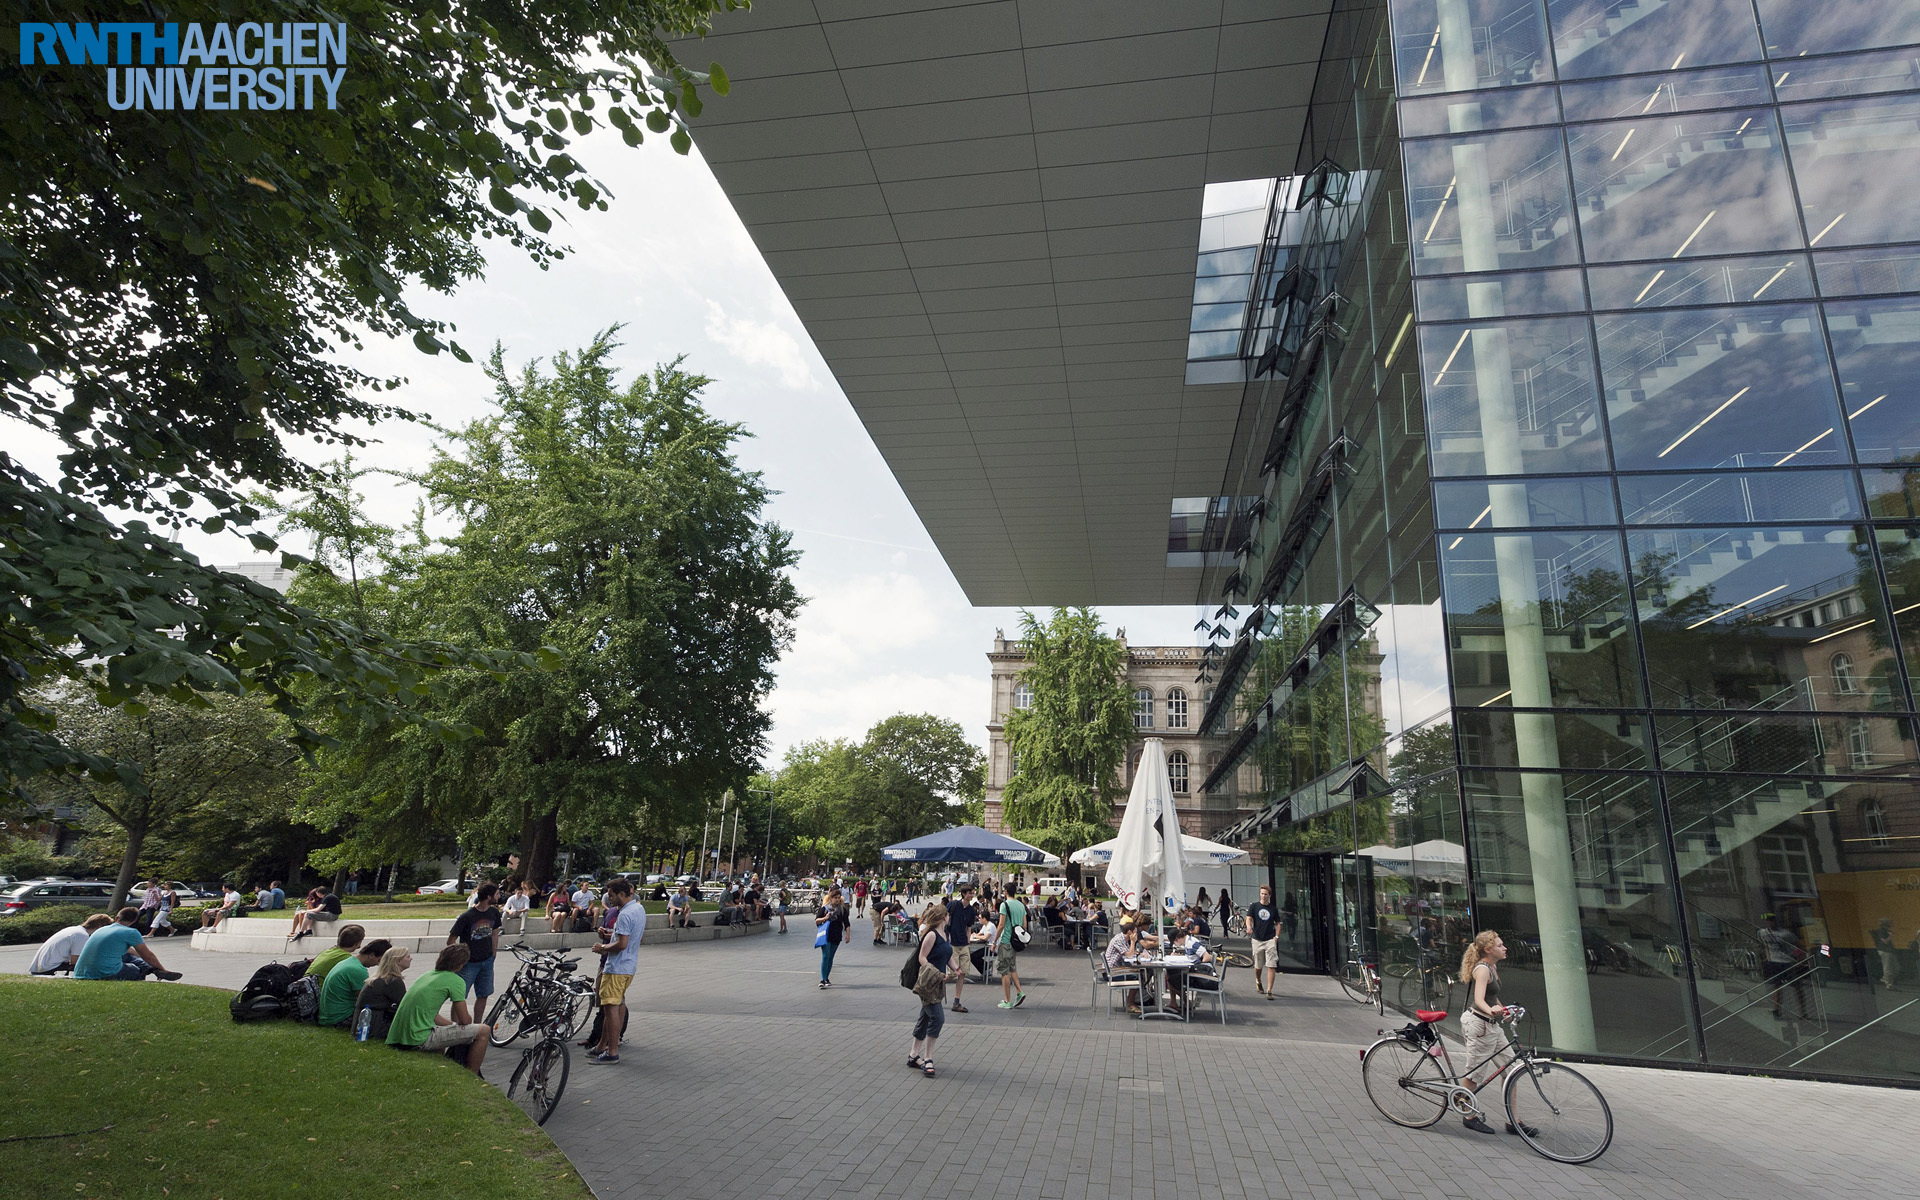
\includegraphics[width = 0.5\textwidth]{Contents/Resources/superc.jpeg}
	\caption[Image (short caption without source)]{Image (detailed caption including source, Source: \cite[1]{Sample.2012})}
	\label{fig:a_image}
\end{figure}

\begin{figure}[htbp]
	\centering
	\begin{subfigure}[t]{0.46\textwidth}
		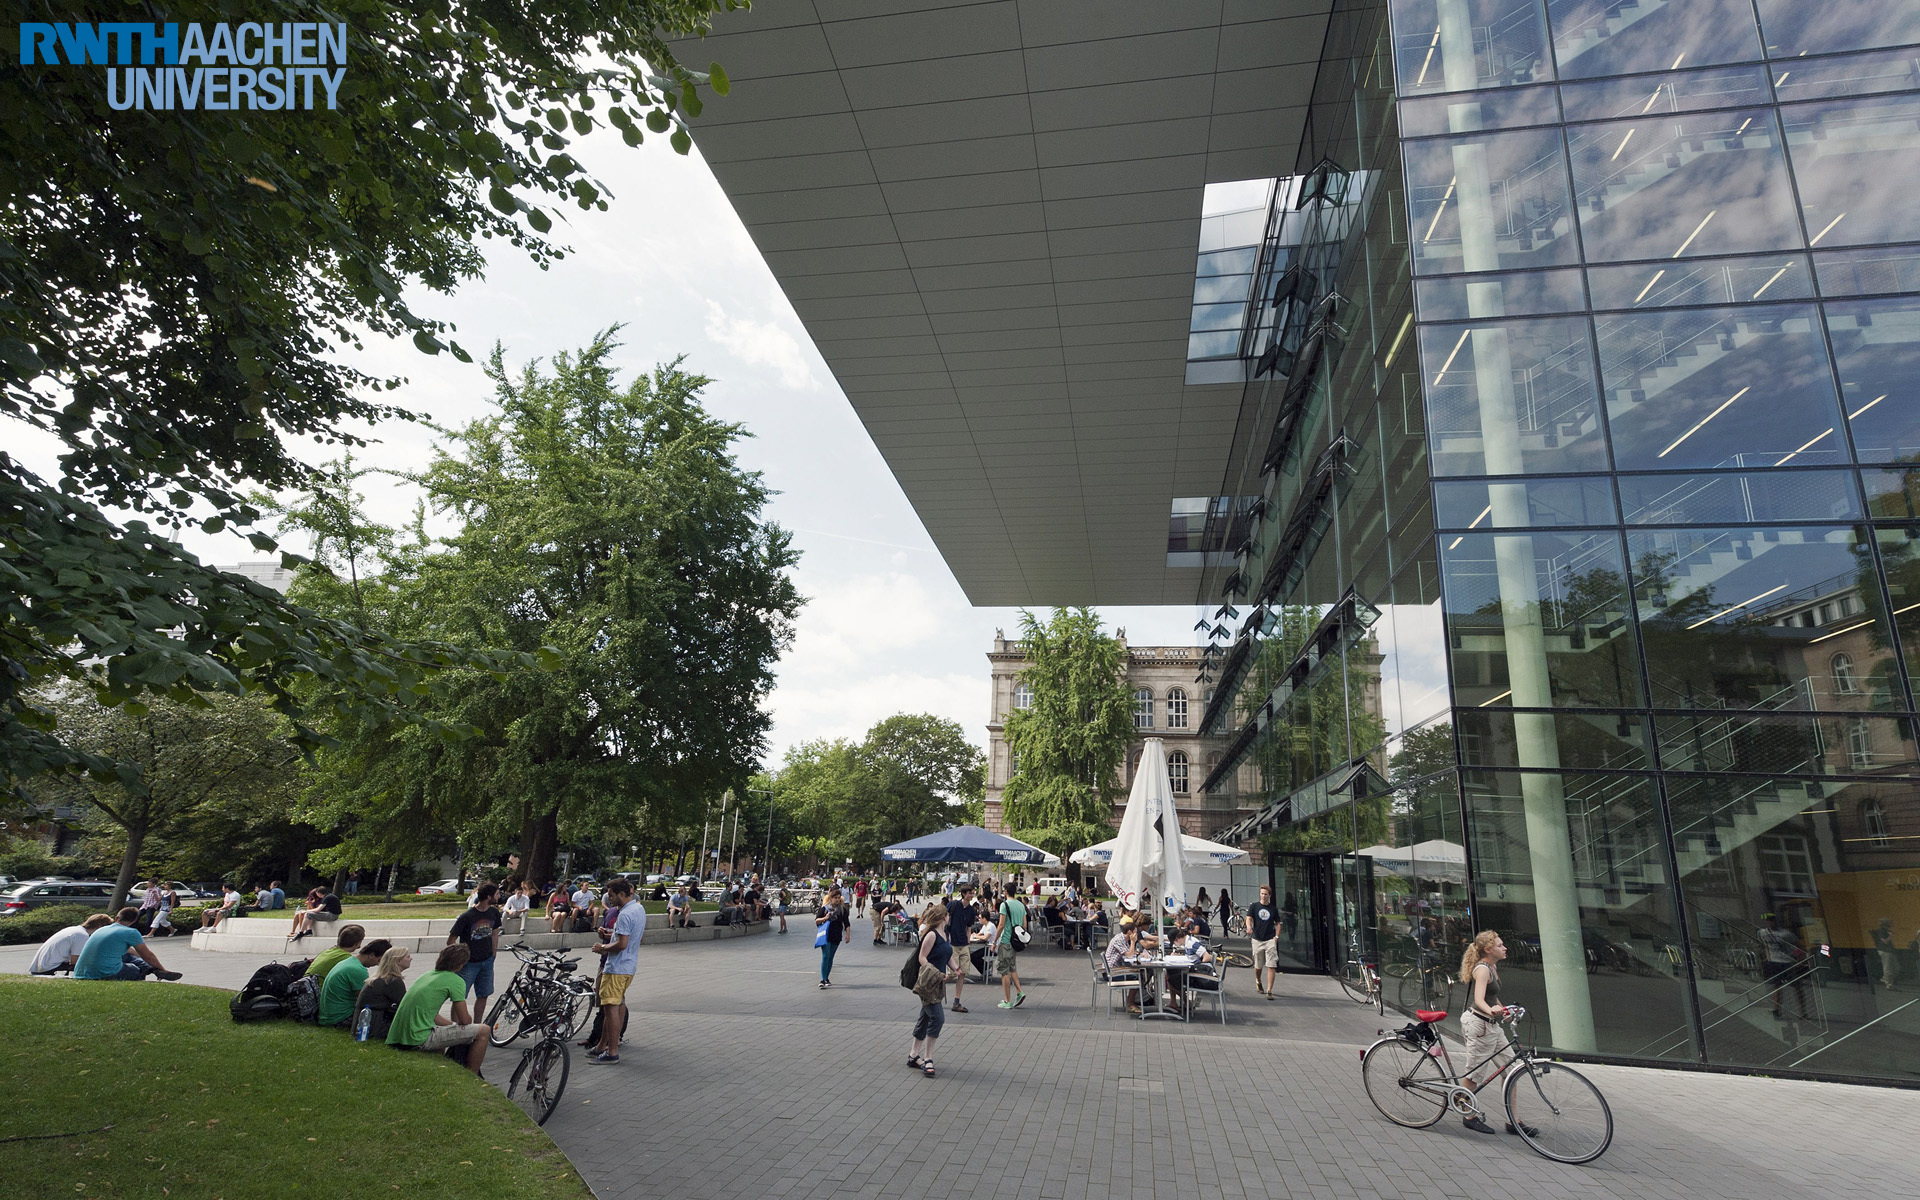
\includegraphics[width = 1\textwidth]{Contents/Resources/superc.jpeg}
		\caption{Image 1}
		\label{fig:image1}
	\end{subfigure}
	\begin{subfigure}[t]{0.46\textwidth}
		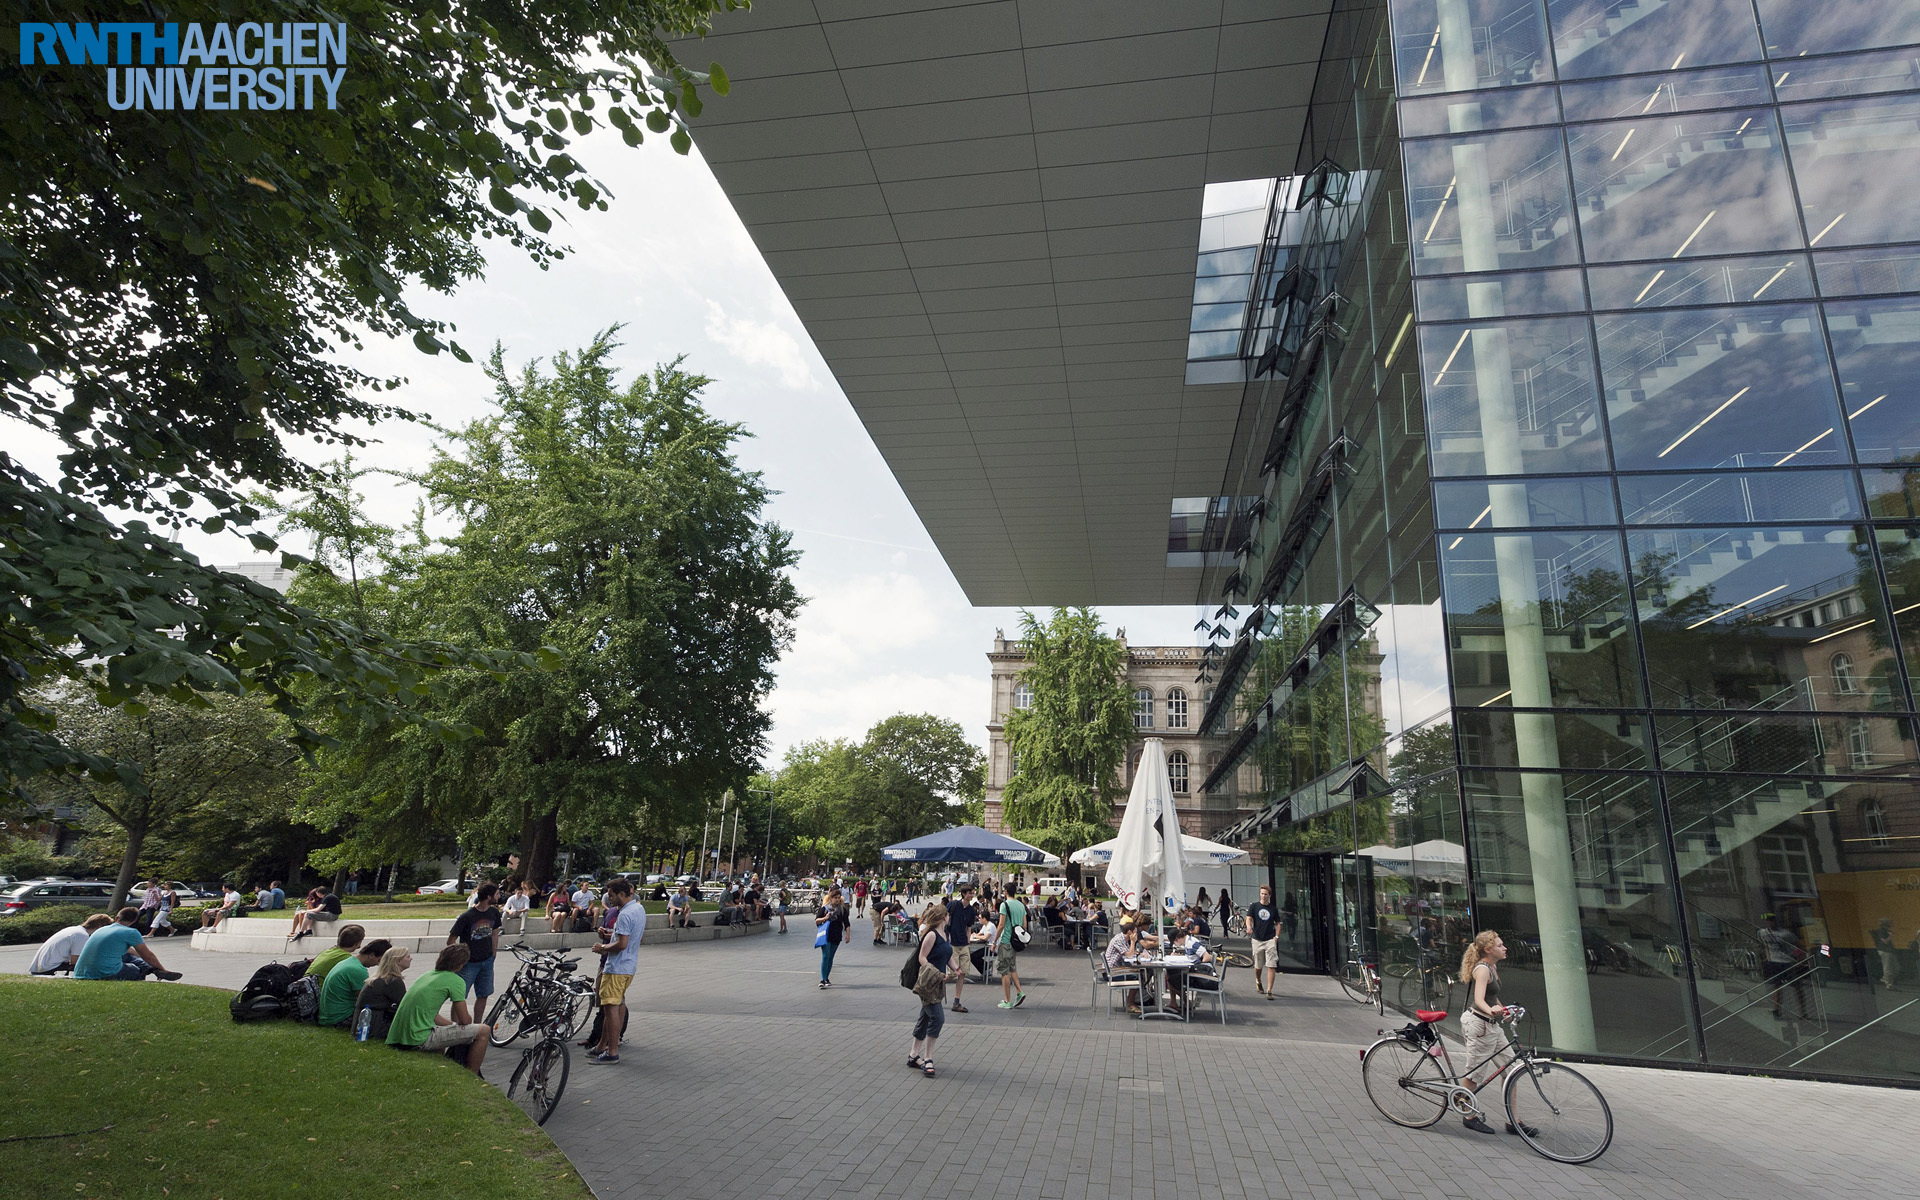
\includegraphics[width = 1\textwidth]{Contents/Resources/superc.jpeg}
		\caption{Image 2}
		\label{fig:image2}
	\end{subfigure}
	\caption[Two images]{Image 1 (a) and Image 2 (b)}
	\label{fig:multiple_images}
\end{figure}

\cleardoublepage
% Section 3 --------------------------------------------------------------
% 		Name of the section
% --------------------------------------------------------------------------
\section{Tables}
\label{sec:tables}

\begin{table}[htbp]
	\centering	
	\caption{Tables with automatic alignment}
		\begin{tabular}{lcr}
	 	\toprule
	 	l & c & r\\
	 	\midrule
		a & b & c\\[0.25em]
		aa & bb & cc\\[0.25em]
		aaa & bbb & ccc\\
		\bottomrule
	\end{tabular}	
	\label{tab:table1}
\end{table}

\begin{table}[htbp]
  \centering
  \caption{Tables aligned to seperators}
    \begin{tabular}{R{4}{3} R{4}{0}}
    \toprule
          \multicolumn{1}{c}{a} & \multicolumn{1}{c}{b}\\
    \midrule
	1,234 & 1234\\
	12,34 & 123\\
	123,4 & 12\\
	1234  & 1\\
    \bottomrule
    \end{tabular}
  \label{tab:table2}
\end{table}

\begin{table}[htbp]
	\centering	
	\caption{Table with multiple cells across various rows and columns}
		\begin{tabular}{lcr}
	 	\toprule
	 	l & c & r\\
	 	\midrule
		\multicolumn{2}{c}{ab} & c\\[0.25em]
		\multirow{2}{*}{aa} & bb & cc\\[0.25em]
		& bbb & ccc\\
		\bottomrule
	\end{tabular}	
	\label{tab:table3}
\end{table}

%\begin{table}[htbp]
%  \centering
%  \caption{multiple sub-tables}
%  \subtable[table 1]{
%    \centering  
%\begin{tabular}{lcr}
%	 	\toprule
%	 	l & c & r\\
%	 	\midrule
%		a & b & c\\[0.25em]
%		aa & bb & cc\\[0.25em]
%		aaa & bbb & ccc\\
%		\bottomrule
%	\end{tabular}	
%  }
%  \subtable[Tabelle 2]{
%    \centering  
%\begin{tabular}{lcr}
%	 	\toprule
%	 	l & c & r\\
%	 	\midrule
%		a & b & c\\[0.25em]
%		aa & bb & cc\\[0.25em]
%		aaa & bbb & ccc\\
%		\bottomrule
%	\end{tabular}	
%  }
%\label{tab:tables}
%\end{table}

\cleardoublepage
% Section 4 --------------------------------------------------------------
% 		Name of the section
% --------------------------------------------------------------------------
\section{Equations}
\label{sec:equations}

\begin{align}
	F = m a 
	\label{eqn:newton_en}
\end{align}


\section{Citation options}

Cite a source: \cite{Sample.2012}\\
Cite a source with a page reference: \cite[12-16]{Sample.2012}\\
Cite multiple Sources: \cites{Samplem.2012}{Samplef.2011}\\
Cite multiple sources with page references: \cites[12-16]{Samplem.2012}[3]{Samplef.2011}\\


% \chapter{Beispielkapitel}
\label{cha:beispielkapitel}
Dieses Beispielkapitel dient der Darstellung häufig verwendeter Elemente in LaTeX wie Aufzählungen, Abbildungen, Tabellen oder Gleichungen. Es hat keinen Anspruch auf Vollständigkeit und kann gerne erweitert werden. Eine ausführliche Beschreibung der LaTeX-Befehle kann der Befehlsübersicht entnommen werden.
Die  Beispiele können kopiert und dann angepasst werden.  
% Abschnitt 1 --------------------------------------------------------------
% 		Name des Abschnittes
% --------------------------------------------------------------------------
\section{Aufzählungen}
\label{sec:aufzaehlungen}

\subsection{Aufzählungen mit Punkten}
\label{aufzaehlung_punkte}

\begin{itemize}
	\item Körper
	\item Bindungselemente
	\item Koppelelemente
\end{itemize}

\subsection{Aufzählungen mit Zahlen}
\label{aufzaehlung_zaheln}

\begin{enumerate}
	\item Körper
	\item Bindungselemente
	\item Koppelelemente
\end{enumerate}

\cleardoublepage
% Abschnitt 2 --------------------------------------------------------------
% 		Name des Abschnittes
% --------------------------------------------------------------------------
\section{Abbildungen}
\label{sec:abbildungen}

\begin{figure}[htbp]
	\centering
		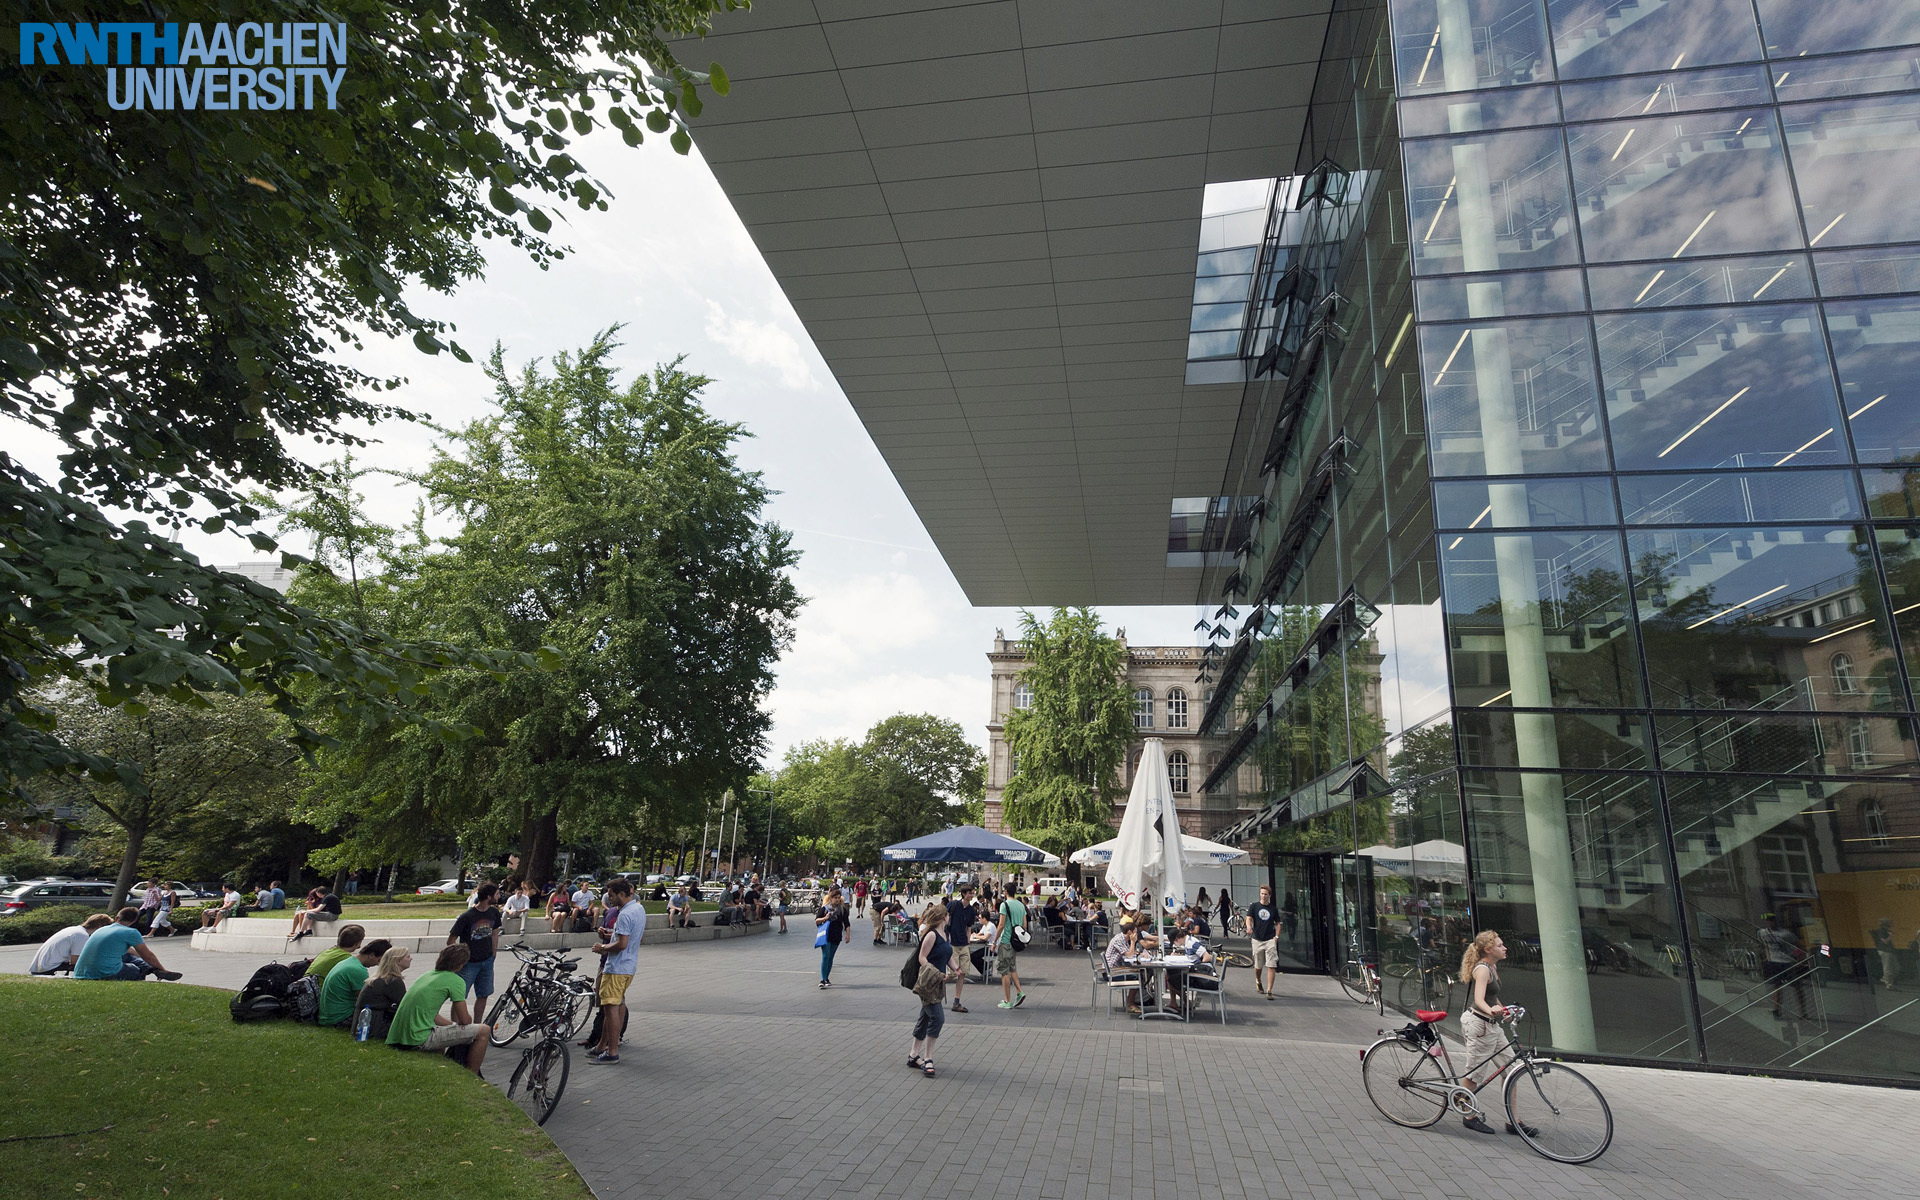
\includegraphics[width = 0.5\textwidth]{Contents/Resources/superc.jpeg}
	\caption[Eine Abbildung (kurze Abbildungsunterschrift ohne Quelle)]{Eine Abbildung (lange Abbildungsunterschrift mit Quelle, Quelle: \cite[1]{Mustermann.2012})}
	\label{fig:eine_abbildung}
\end{figure}

\begin{figure}[htbp]
	\centering
	\begin{subfigure}[t]{0.46\textwidth}
		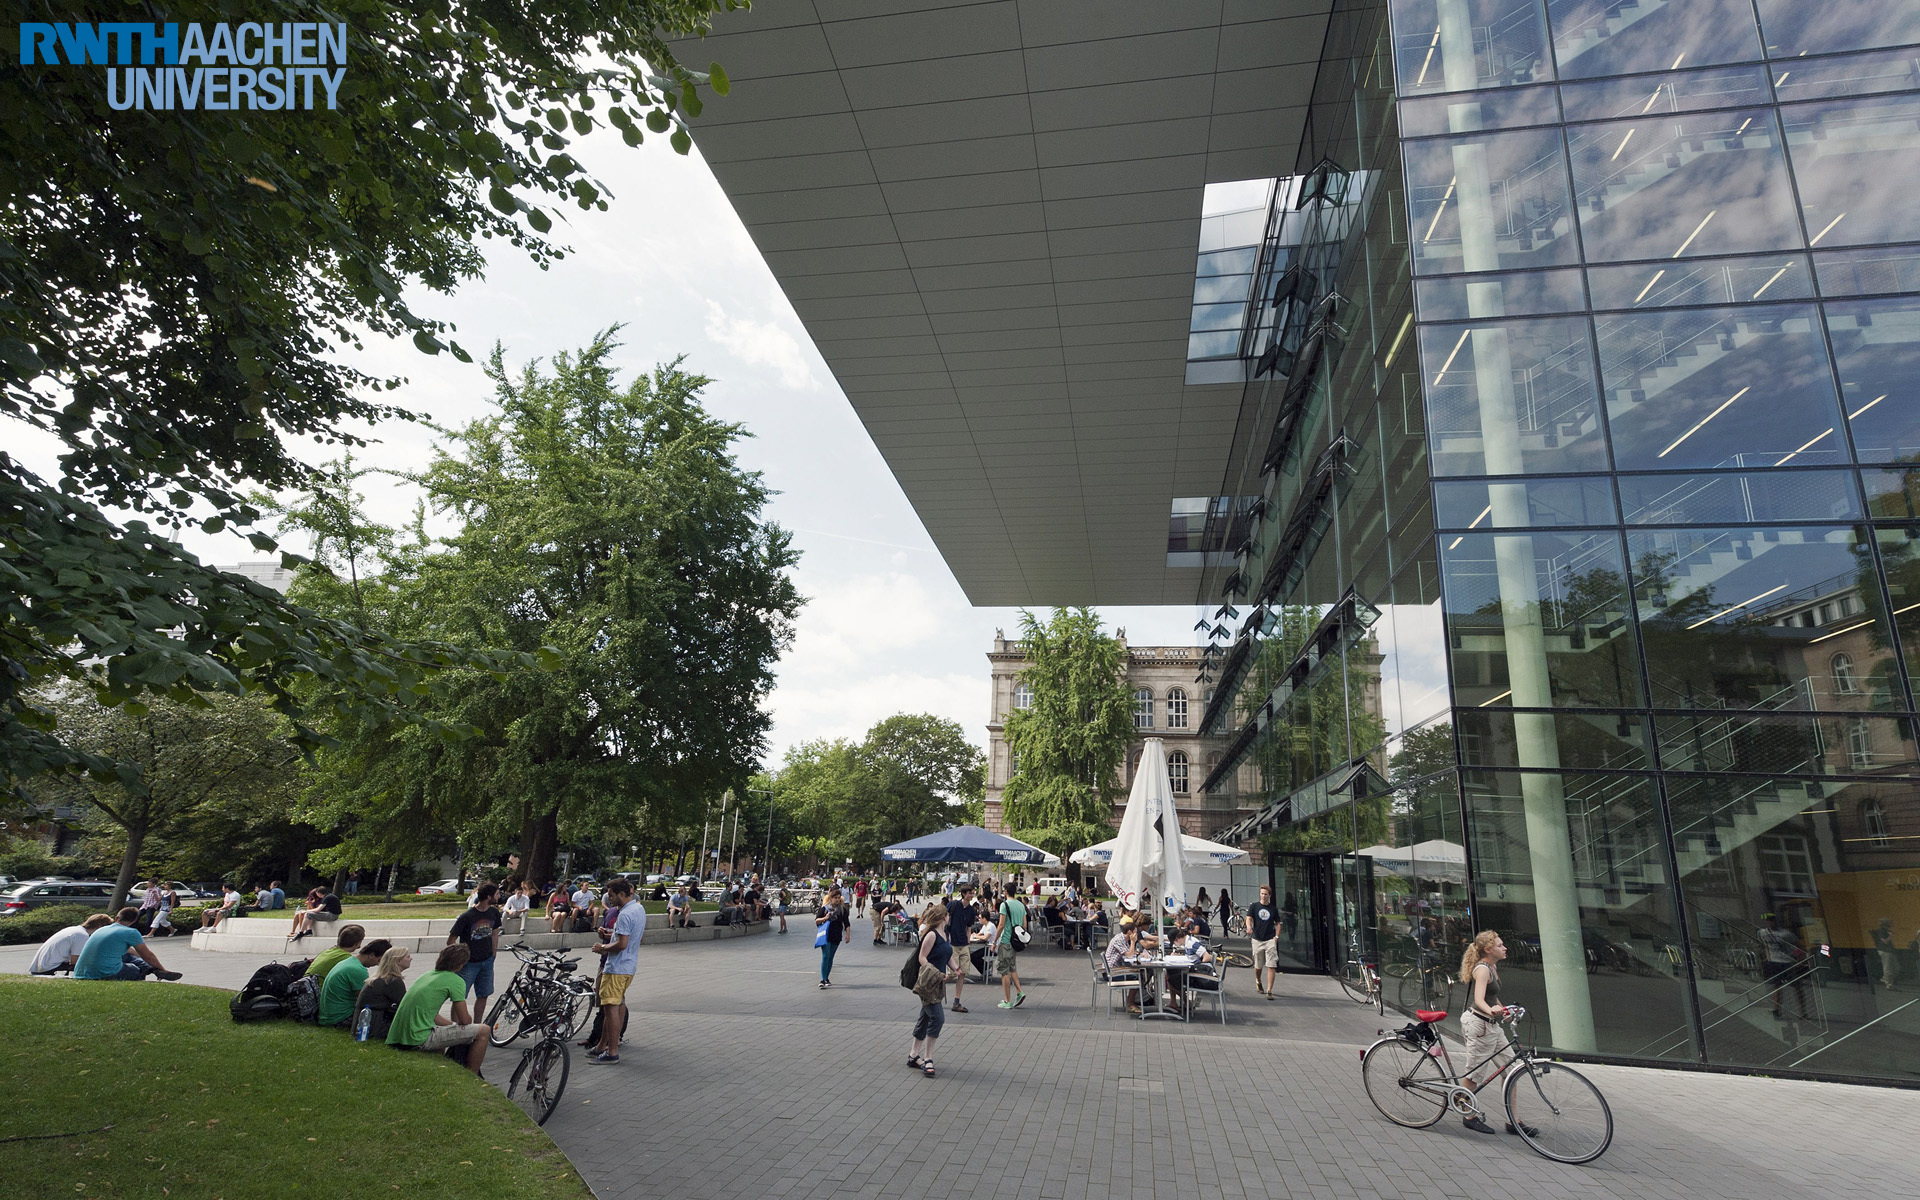
\includegraphics[width = 1\textwidth]{Contents/Resources/superc.jpeg}
		\caption{Bild 1}
		\label{fig:bild1}
	\end{subfigure}
	\begin{subfigure}[t]{0.46\textwidth}
		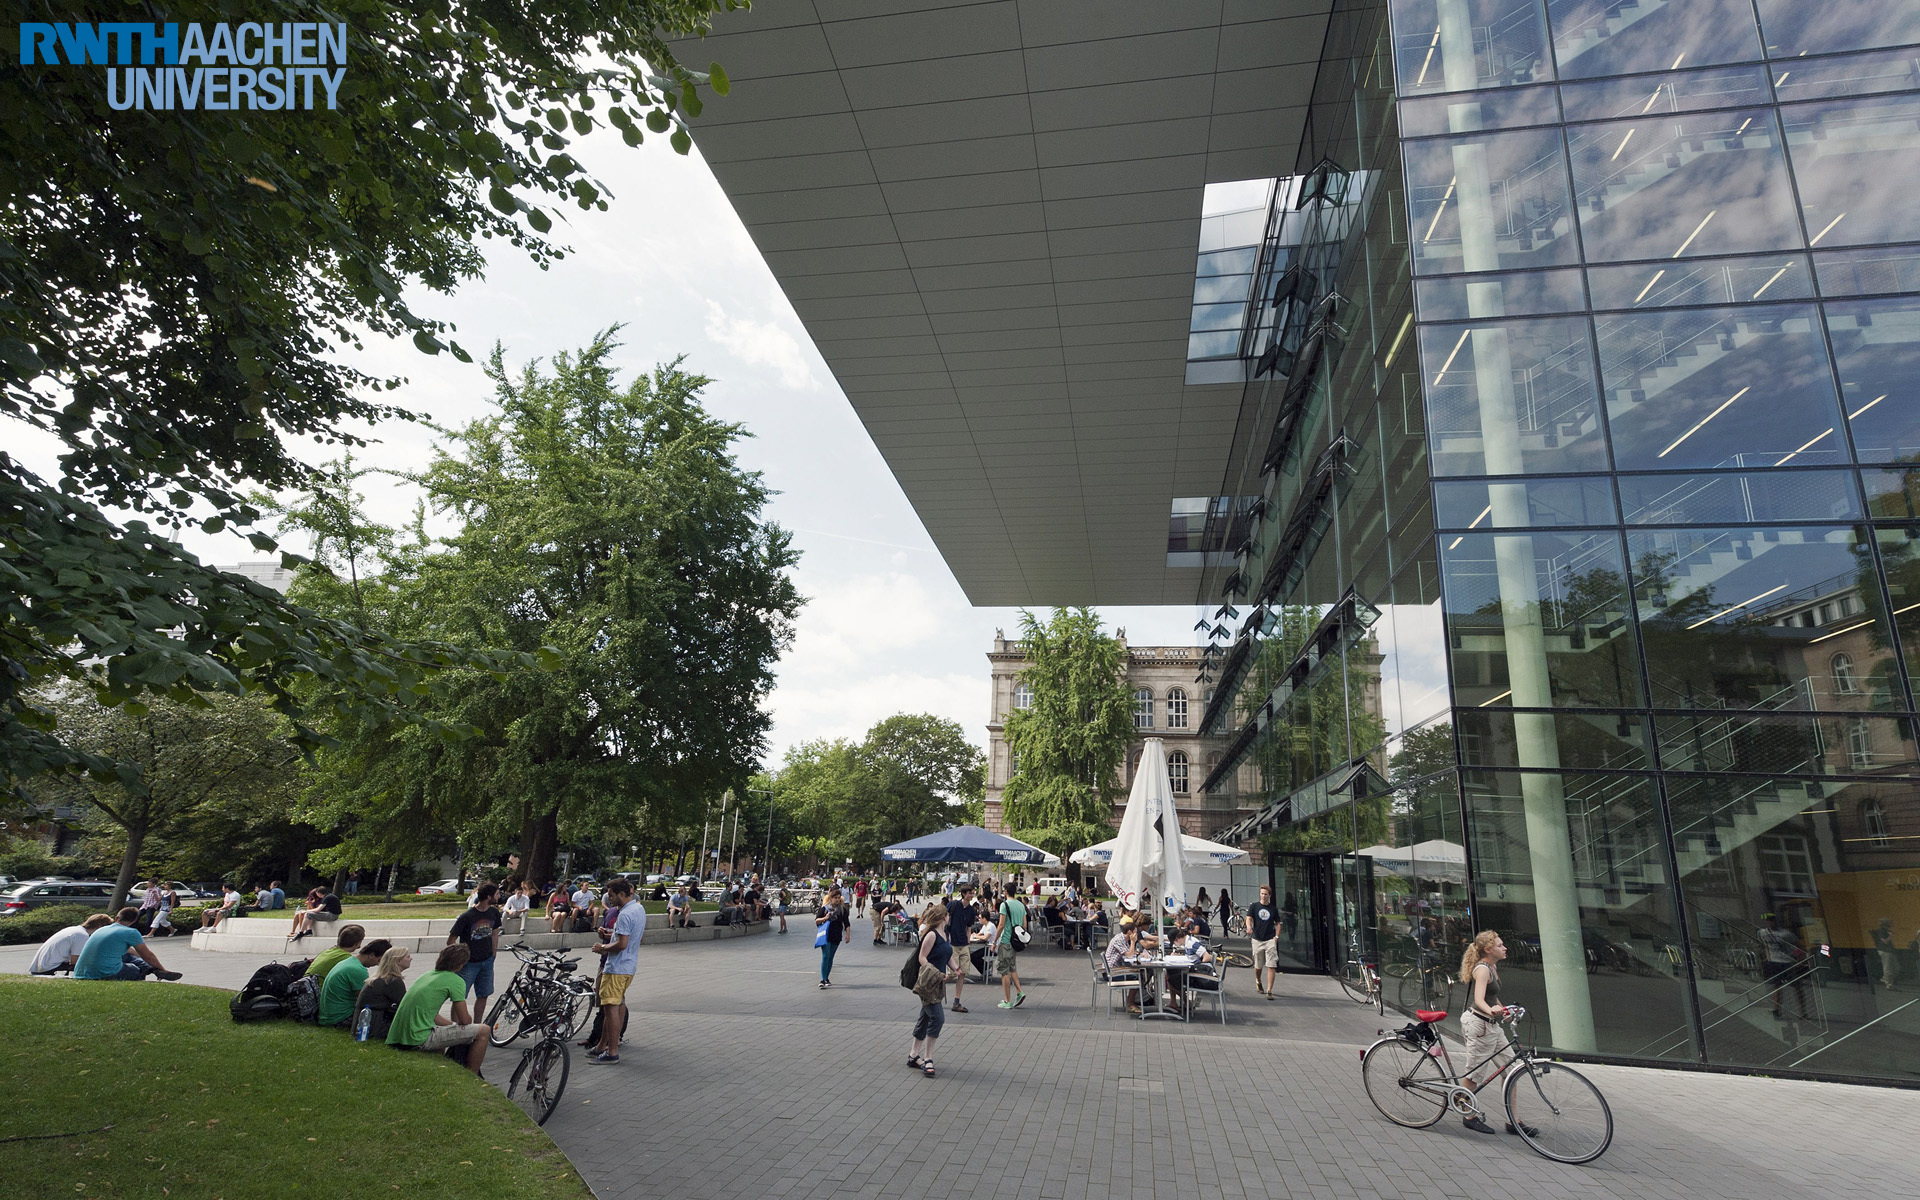
\includegraphics[width = 1\textwidth]{Contents/Resources/superc.jpeg}
		\caption{Bild 2}
		\label{fig:bild2}
	\end{subfigure}
	\caption[Zwei Abbildungen]{Bild 1 (a) und Bild 2 (b)}
	\label{fig:mehrere_abbildungen}
\end{figure}

\cleardoublepage
% Abschnitt 3 --------------------------------------------------------------
% 		Name des Abschnittes
% --------------------------------------------------------------------------
\section{Tabellen}
\label{sec:tabellen}

\begin{table}[htbp]
	\centering	
	\caption{Tabelle mit automatischer Ausrichtung}
		\begin{tabular}{lcr}
	 	\toprule
	 	l & c & r\\
	 	\midrule
		a & b & c\\[0.25em]
		aa & bb & cc\\[0.25em]
		aaa & bbb & ccc\\
		\bottomrule
	\end{tabular}	
	\label{tab:tabelle1}
\end{table}

\begin{table}[htbp]
  \centering
  \caption{Tabelle mit Ausrichtung an Trennungszeichen}
    \begin{tabular}{R{4}{3} R{4}{0}}
    \toprule
          \multicolumn{1}{c}{a} & \multicolumn{1}{c}{b}\\
    \midrule
	1,234 & 1234\\
	12,34 & 123\\
	123,4 & 12\\
	1234  & 1\\
    \bottomrule
    \end{tabular}
  \label{tab:tabelle2}
\end{table}

\begin{table}[htbp]
	\centering	
	\caption{Tabelle mit Zellen über mehrere Zeilen oder Spalten}
		\begin{tabular}{lcr}
	 	\toprule
	 	l & c & r\\
	 	\midrule
		\multicolumn{2}{c}{ab} & c\\[0.25em]
		\multirow{2}{*}{aa} & bb & cc\\[0.25em]
		& bbb & ccc\\
		\bottomrule
	\end{tabular}	
	\label{tab:tabelle3}
\end{table}

%\begin{table}[htbp]
%  \centering
%  \caption{Mehrere Untertabellen}
%  \subtable[Tabelle 1]{
%    \centering  
%\begin{tabular}{lcr}
%	 	\toprule
%	 	l & c & r\\
%	 	\midrule
%		a & b & c\\[0.25em]
%		aa & bb & cc\\[0.25em]
%		aaa & bbb & ccc\\
%		\bottomrule
%	\end{tabular}	
%  }
%  \subtable[Tabelle 2]{
%    \centering  
%\begin{tabular}{lcr}
%	 	\toprule
%	 	l & c & r\\
%	 	\midrule
%		a & b & c\\[0.25em]
%		aa & bb & cc\\[0.25em]
%		aaa & bbb & ccc\\
%		\bottomrule
%	\end{tabular}	
%  }
%\label{tab:tabellen}
%\end{table}

\cleardoublepage
% Abschnitt 4 --------------------------------------------------------------
% 		Name des Abschnittes
% --------------------------------------------------------------------------
\section{Gleichungen}
\label{sec:gleichungen}

\begin{align}
	F = m a 
	\label{eqn:newton}
\end{align}


\section{Anführungszeichen}
\label{sec:anfuehrungszeichen}
Es gibt mehrere Möglichkeiten deutsche Anführungszeichen einzufügen:\\
\glqq test\grqq\\
"`test"'\\

\section{Zitationen}

Zitation einer Quelle: \cite{Mustermann.2012}\\
Zitation einer Quelle mit Seitenangabe: \cite[12-16]{Mustermann.2012}\\
Zitation mehrerer Quellen: \cites{Mustermann.2012}{Musterfrau.2011}\\
Zitation mehrerer Quellen mit Seitenangabe: \cites[12-16]{Mustermann.2012}[3]{Musterfrau.2011}\\



% \chapter{Zusammenfassung}
\label{cha:zusammenfassung}


%
% \chapter{Outlook}\label{cha:outlook}


%       EXTRAS
%		x Title page
%		- Half title??
%		- Issue [last]
%		x Statutory declaration
%		- (Preface)
%		x Table of contents
%		- List of abbreviations
%		- List of symbols

%       MAIN CHAPTERS
%		- Introduction
%		- Chapters
%		- Summary
%		- Outlook

%       EXTRAS
%		- List of literature
%		- List of illustrations
%		- List of tables
%		- Appendix

%%%%%%%%%%%%%%%%%%%%%%%%%%%%%%%%%%%%%%%%%%%%%%%%%%%%%%%%%%%%%%%%%%%%%%%%%%%%
%%%%%%%%%%%%%%%%%%%%%%%%%%%%%%%%%%%%%%%%%%%%%%%%%%%%%%%%%%%%%%%%%%%%%%%%%%%%
%%%%%%%%%%%%%%%%%%%%%%%%%%%%%%%%%%%%%%%%%%%%%%%%%%%%%%%%%%%%%%%%%%%%%%%%%%%%

\pagenumbering{Roman}
% --------------------------------------------------------------------------
%		Literaturverzeichnis / List of literature	
% -------------------------------------------------------------------------- 
\printbibliography[heading=bibintoc]

% --------------------------------------------------------------------------
%		Tabellenverzeichnis / List of tables
% -------------------------------------------------------------------------- 
\listoftables						% Tabellenverzeichnis / List of tables
\cleardoublepage

% --------------------------------------------------------------------------
%		Abbildungsverzeichnis / Register of illustrations
% -------------------------------------------------------------------------- 
\listoffigures						% Abbildungsverzeichnis / Register of illustrations
\cleardoublepage

% --------------------------------------------------------------------------
%		Anhang / Attachment
%
%		Der Anhnag enthält weitere Dokumente, welche nicht direkt zur Arbeit
%		gehören oder aus Platzgründen ausgelagert werden müssen. Die Kapitel
%		des Anhangs werden mit Großbuchstaben bezeichnet
%
%		The attachment contains further documents which are not related to work directly or
%		had to be outsourced due to a lack of space. The different chapters of the attachment 
%		are labeled with a captital letter.
% -------------------------------------------------------------------------- 
\appendix

% Inhalt des Anhangs (Beispiel) / List of contents of attachment (Example) 
\chapter{Illustrations}\label{cha:anhang_abbildungen}

\cleardoublepage
\chapter{Tables}\label{cha:anhang_tabellen}
\cleardoublepage

\backmatter
\end{document}